% Preamble
\documentclass[11pt]{article}

% Packages
\usepackage{amsmath}
\usepackage[a4paper, margin=0.5in]{geometry}
\usepackage{graphicx} % daj an 1in jak chcesz normalniejszy margines, ale kod mi się w linii nie mieści :P
\usepackage[utf8]{inputenc}
\usepackage[T1]{fontenc}
\usepackage[polish]{babel}
\usepackage{float}
\usepackage{hyperref}
\usepackage{cleveref}
\usepackage{subfigure}

\title{Zadanie 2. Lokalne przeszukiwanie}
\author{Oskar Kiliańczyk 151863 \& Wojciech Kot 151876}
\date{}

% Document
\begin{document}

\maketitle
\newpage

\section{Opis zadania}\label{sec:opis-zadania}
Zadanie polega na implementacji lokalnego przeszukiwania w wersjach stromej (steepest) i zachłannej (greedy), z dwoma różnym rodzajami sąsiedztwa,
startując albo z rozwiązań losowych, albo z rozwiązań uzyskanych za pomocą jednej z heurystyk opracowanych w ramach poprzedniego zadania.
W sumie 8 kombinacji --- wersji lokalnego przeszukiwania.
Jako punkt odniesienia należy zaimplementować algorytm losowego błądzenia, który w każdej iteracji wykonuje losowo wybrany ruch (niezależnie od jego oceny) i zwraca najlepsze znalezione w ten sposób rozwiązanie.
Algorytm ten powinien działać w takim samym czasie jak średnio najwolniejsza z wersji lokalnego przeszukiwania.

\subsection{Sąsiedztwa}\label{subsec:sasiedztwa}
W przypadku rozważanego problemu potrzebne będą dwa typy ruchów:
\begin{itemize}
\item ruchy zmieniające zbiory wierzchołków tworzące dwa cykle,
\item ruchy wewnątrztrasowe, które jedynie zmieniają kolejność wierzchołków na trasie.
\end{itemize}
Stosujemy dwa rodzaje ruchów wewnątrztrasowych (jeden albo drugi, stąd dwa rodzaje sąsiedztwa).
Jeden to wymiana dwóch wierzchołków wchodzących w skład trasy, drugi to wymiana dwóch krawędzi.
Dla ruchów wewnątrz cykli wykonujemy lokalne zamiany elementów w obrębie jednej ścieżki.

\subsection{Randomizacja kolejności przeglądania dla algorytmów zachłannych}\label{subsec:randomizacja-kolejnosci-przegladania-dla-algorytmow-zachannych}
W obu wersjach algorytmów zachłannych stosujemy randomizację wyboru.
Tworzymy listę możliwych par punktów do zamiany wewnątrz cyklu lub między dwoma cyklami.
Losowo przetasowujemy te możliwe pary, dzięki czemu kolejność przetwarzania nie jest deterministyczna.
Wybieramy pary do wymiany aż nie znajdziemy takiej, dla której zamiana daje poprawę funkcji celu.
Jeśli taka istnieje, przeprowadzamy zamianę i powtarzamy procedurę, jeśli nie ma takiej pary - kończymy przetwarzanie.

\subsection{Algorytmy startowe}\label{subsec:algorytmy-startowe}

Napisane na potrzebę tego zadania algorytmy wykorzystują dwa różne algorytmy startowe
(generujące rozwiązanie bazowe, które napisane obecnie algorytmy lokalnego przeszukiwania będą ulepszać).
Pierwszy z nich, nazwaliśmy randomstart - zwraca on dwa losowe zbiory wierzchołków, tworząc w pełni losowo wygenerowane bazowe rozwiązanie, które będzie relatywnie proste do polepszenia.
Drugi z nich natomiast, to nasz własny algorytm (nie zaproponowany w zadaniu) który łączył heurystykę żalu z zachłannym podziałem wierzchołków na dwa podzbiory.


\section{Opisy algorytmów}\label{sec:opisy-alg}

\subsection{Opisy dostępnych ruchów}

\subsubsection{Obliczanie zmiany kosztu przy zamianie wierzchołków}

Dla dwóch pozycji $i$ i $j$ w cyklu:
\begin{enumerate}
    \item Jeśli $i$ i $j$ są sąsiadami:
    \begin{enumerate}
        \item Wyznacz wierzchołki poprzedzające i następujące po parze $(i, j)$.
        \item Oblicz sumę długości krawędzi przed i po zamianie miejscami $i$ i $j$.
    \end{enumerate}
    \item W przeciwnym wypadku:
    \begin{enumerate}
        \item Wyznacz wierzchołki poprzedzające i następujące po $i$ i po $j$.
        \item Oblicz sumę długości czterech krawędzi: przed i po zamianie $i$ i $j$.
    \end{enumerate}
    \item Zwróć różnicę: \textit{nowy koszt} $-$ \textit{stary koszt}.
\end{enumerate}

\subsubsection{Obliczanie zmiany kosztu przy zamianie krawędzi}

Dla dwóch pozycji $i$ i $j$ w cyklu:
\begin{enumerate}
    \begin{enumerate}
        \item Wyznacz wierzchołki poprzedzające i następujące po $i$ i po $j$.
        \item Oblicz sumę długości krawędzi: przed zamianą $i$ i $j$.
        \begin{enumerate}
            \item długość $i-1 -> i$ + długość $j -> j+1$
        \end{enumerate}
        \item Oblicz sumę długości po zamianie krawędzi:
        \begin{enumerate}
            \item długość $i-1 -> j-1$ + długość $i -> j$
        \end{enumerate}
    \end{enumerate}
    \item Zwróć różnicę: \textit{nowy koszt} $-$ \textit{stary koszt}.
\end{enumerate}

\subsecion{Algorytmy}

\subsubsection{Zachłanny}\label{subsec:zachanny}

\begin{enumerate}
    \item Dla każdego z dwóch cykli:
    \begin{enumerate}
        \item Dopóki możliwa jest poprawa*:
        \begin{enumerate}
            \item Wygeneruj listę możliwych par wierzchołków $(i, j)$ wewnątrz cyklu.
            \item Permutuj listę i sprawdzaj kolejne pary:
            \begin{enumerate}
                \item Oblicz zmianę kosztu po ruchu lokalnym (zamiana wierzchołków lub odwrócenie fragmentu).
                \item Jeśli koszt się zmniejsza, wykonaj ruch.
                \item Przerwij sprawdzanie i wróć na początek pętli (*).
            \end{enumerate}
        \end{enumerate}
    \end{enumerate}

    \item Dopóki możliwa jest poprawa międzycyklowa:
    \begin{enumerate}
        \item Wygeneruj losową permutację par wierzchołków $(i, j)$ z dwóch cykli.
        \item Dla każdej pary:
        \begin{enumerate}
            \item Oblicz zmianę kosztu po zamianie wierzchołków między cyklami.
            \item Jeśli koszt się zmniejsza, wykonaj zamianę i zaznacz poprawę.
        \end{enumerate}
        \item Jeżeli wykonano jakąkolwiek zamianę, wróć do lokalnej optymalizacji (punkt 1).
    \end{enumerate}

    \item Zakończ, gdy nie ma już żadnych lokalnych ani międzycyklowych poprawek.
\end{enumerate}


\subsubsection{Steepest}\label{subsec:steepest}

\begin{enumerate}
  \item Dopóki możliwa jest poprawa:
  \begin{enumerate}
    \item Przeszukaj wszystkie możliwe modyfikacje ścieżek:
    \begin{itemize}
      \item zmiany lokalne w jednej ścieżce (zamiana dwóch wierzchołków lub odwrócenie fragmentu),
      \item wymiany wierzchołków między ścieżkami.
    \end{itemize}
    \item Wybierz modyfikację dającą największą poprawę.
    \item Wprowadź ją do odpowiedniej ścieżki lub ścieżek.
  \end{enumerate}
  \item Zwróć ulepszone ścieżki.
\end{enumerate}

\subsubsection{Random Traverse}

\begin{enumerate}
    \item Zainicjuj wartość rozwiązania jako 0.
    \item Dopóki czas przetwarzania jest mniejszy niż limit:
    \begin{enumerate}
        \item Wybierz losowy ruch z całej puli dostępnych ruchów.
        \item Oblicz zmianę funkcji celu dla tego ruchu.
        \item Wykonaj ruch i dodaj zmianę do ogólnej wartości rozwiązania.
        \item Jeśli wartość rozwiązania jest obecnie najlepsza:
        \begin{enumerate}
            \item Zapisz rozwiązanie jako najlepszego
        \end{enumerate}
    \end{enumerate}
    \item Po upływie czasu zwróć najlepsze znalezione rozwiązanie.
\end{enumerate}


\section{Wyniki}\label{sec:wyniki}

\subsection{Tabela wynikowa}\label{subsec:tabela-wynikowa}

% Tabela 1: kroA200.tsp z randomstart
\begin{table}[ht]
\centering
\resizebox{\textwidth}{!}{
\begin{tabular}{|l|l|r|r|r|r|r|r|}
\hline
\textbf{Instance} & \textbf{Algorytm} & \textbf{Best} & \textbf{Avg} & \textbf{Worst} & \textbf{Avg Time} & \textbf{Best Diff} & \textbf{Avg Diff} \\
\hline
\texttt{kroA200} & \texttt{greedy\_edge} & 38683 & 43477.2 & 46597 & 0.0911878 & 323996 & 297870 \\
\texttt{kroA200} & \texttt{greedy\_vertex} & 65591 & 79580.1 & 89485 & 0.227998 & 291579 & 262294 \\
\texttt{kroA200} & \texttt{steepest\_edge} & 38261 & 42868 & 49455 & 1.38019 & 335537 & 298626 \\
\texttt{kroA200} & \texttt{steepest\_vertex} & 65990 & 79327.8 & 91208 & 2.42133 & 300881 & 263108 \\
\texttt{kroA200} & \texttt{random} & 301648 & 332569 & 354465 & 2.42166 & 38018 & 8544.31 \\
\hline
\end{tabular}
}
\caption{Wyniki dla \texttt{kroA200} z algorytmem \texttt{randomstart}}
\end{table}

% Tabela 2: kroA200.tsp z split_paths_regret_TSP
\begin{table}[ht]
\centering
\resizebox{\textwidth}{!}{
\begin{tabular}{|l|l|r|r|r|r|r|r|}
\hline
\textbf{Instance} & \textbf{Algorytm} & \textbf{Best} & \textbf{Avg} & \textbf{Worst} & \textbf{Avg Time} & \textbf{Best Diff} & \textbf{Avg Diff} \\
\hline
\texttt{kroA200} & \texttt{greedy\_edge} & 30293 & 32567.1 & 37008 & 0.0146494 & 1159 & 203.38 \\
\texttt{kroA200} & \texttt{greedy\_vertex} & 30310 & 32608.6 & 36369 & 0.022078 & 2613 & 285.68 \\
\texttt{kroA200} & \texttt{steepest\_edge} & 30426 & 32421.1 & 36148 & 0.0430189 & 3109 & 479.23 \\
\texttt{kroA200} & \texttt{steepest\_vertex} & 30293 & 32475.8 & 37008 & 0.0496467 & 2552 & 324.68 \\
\texttt{kroA200} & \texttt{random} & 30293 & 33024.9 & 36098 & 2.42141 & 0 & 0 \\
\hline
\end{tabular}
}
\caption{Wyniki dla \texttt{kroA200} z naszym algorytmem}
\end{table}

% Tabela 3: kroB200.tsp z randomstart
\begin{table}[ht]
\centering
\resizebox{\textwidth}{!}{
\begin{tabular}{|l|l|r|r|r|r|r|r|r|}
\hline
\textbf{Instance} & \textbf{Algorytm} & \textbf{Best} & \textbf{Avg} & \textbf{Worst} & \textbf{Avg Time} & \textbf{Best Diff} & \textbf{Avg Diff} \\
\hline
\texttt{kroB200} & \texttt{greedy\_edge} & 38866 & 43465.6 & 46581 & 0.0910784 & 321463 & 291367 \\
\texttt{kroB200} & \texttt{greedy\_vertex} & 70839 & 78826.1 & 88908 & 0.232368 & 291703 & 253942 \\
\texttt{kroB200} & \texttt{steepest\_edge} & 38556 & 43203.3 & 48639 & 1.36221 & 313027 & 291400 \\
\texttt{kroB200} & \texttt{steepest\_vertex} & 67856 & 78534 & 90919 & 2.35443 & 280540 & 254883 \\
\texttt{kroB200} & \texttt{random} & 295224 & 324648 & 351050 & 2.35485 & 38466 & 8461.69 \\
\hline
\end{tabular}
}
\caption{Wyniki dla \texttt{kroB200} z algorytmem \texttt{randomstart}}
\end{table}

% Tabela 4: kroB200.tsp z split_paths_regret_TSP
\begin{table}[ht]
\centering
\resizebox{\textwidth}{!}{
\begin{tabular}{|l|l|r|r|r|r|r|r|}
\hline
\textbf{Instance} & \textbf{Algorytm} & \textbf{Best} & \textbf{Avg} & \textbf{Worst} & \textbf{Avg Time} & \textbf{Best Diff} & \textbf{Avg Diff} \\
\hline
\texttt{kroB200} & \texttt{greedy\_edge} & 31009 & 33192.1 & 36480 & 0.0174221 & 3629 & 501.29 \\
\texttt{kroB200} & \texttt{greedy\_vertex} & 31178 & 33141.9 & 36479 & 0.0225539 & 2879 & 330.03 \\
\texttt{kroB200} & \texttt{steepest\_edge} & 31133 & 32820.3 & 36479 & 0.0346969 & 4046 & 495.55 \\
\texttt{kroB200} & \texttt{steepest\_vertex} & 31368 & 33197.1 & 36010 & 0.0385854 & 2879 & 254.42 \\
\texttt{kroB200} & \texttt{random} & 31526 & 33517.7 & 36555 & 2.35449 & 0 & 0 \\
\hline
\end{tabular}
}
\caption{Wyniki dla \texttt{kroB200} z naszym algorytmem}
\end{table}





\subsection{Wizualizacja wyników}\label{subsec:wizualizacja-wynikow}

\subsubsection{Algorytm wymiany krawędzi (zachłanny)}
\begin{figure}[H]
    \centering
    % --- Pierwszy rząd ---
    \begin{minipage}[t]{0.45\textwidth}
        \centering
        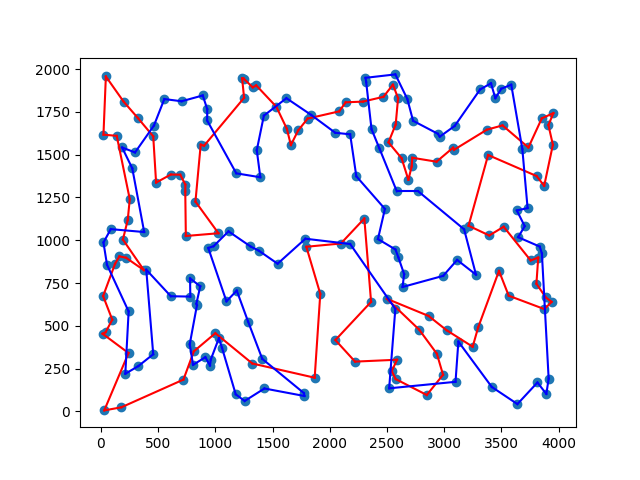
\includegraphics[width=\linewidth]{best_paths/kroA200/traverse_greedy_edge/randomstart}
        \caption{kroA200, losowy start}
    \end{minipage}
    \hfill
    \begin{minipage}[t]{0.45\textwidth}
        \centering
        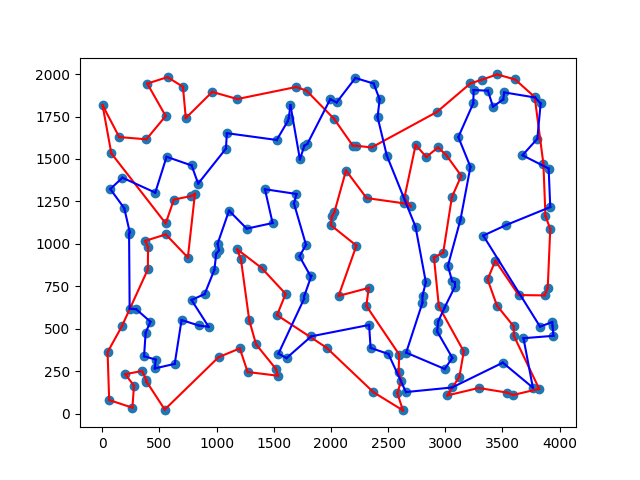
\includegraphics[width=\linewidth]{best_paths/kroB200/traverse_greedy_edge/randomstart}
        \caption{kroB200, losowy start}
    \end{minipage}

    \vspace{0.5cm}

    % --- Drugi rząd ---
    \begin{minipage}[t]{0.45\textwidth}
        \centering
        \includegraphics[width=\linewidth]{best_paths/kroA200/traverse_greedy_edge/split_paths_regret_TSP}
        \caption{kroA200, własny algorytm startowy}
    \end{minipage}
    \hfill
    \begin{minipage}[t]{0.45\textwidth}
        \centering
        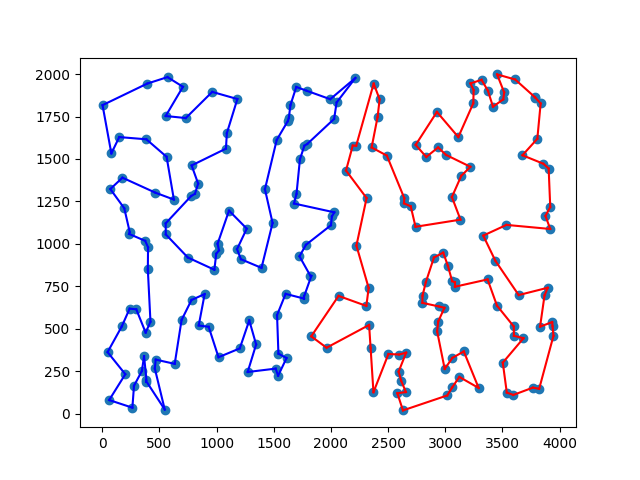
\includegraphics[width=\linewidth]{best_paths/kroB200/traverse_greedy_edge/split_paths_regret_TSP}
        \caption{kroB200, własny algorytm startowy}
    \end{minipage}
    \label{fig:minipage-greedy-edge}
\end{figure}

\subsubsection{Algorytm wymiany wierzchołków (zachłanny)}
\begin{figure}[H]
    \centering
    % --- Pierwszy rząd ---
    \begin{minipage}[t]{0.45\textwidth}
        \centering
        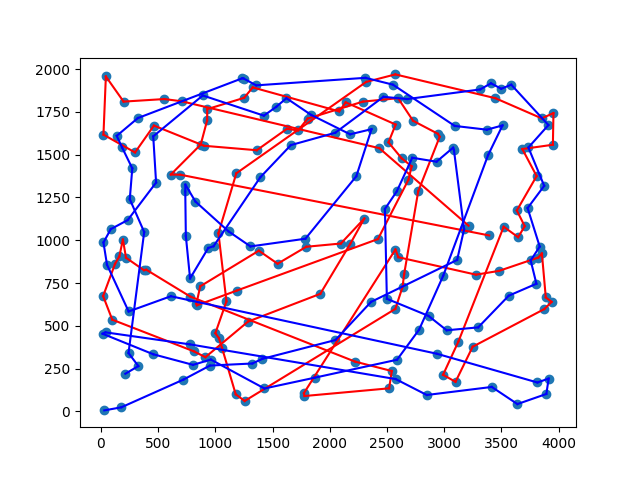
\includegraphics[width=\linewidth]{best_paths/kroA200/traverse_greedy_vertex/randomstart}
        \caption{kroA200, losowy start}
    \end{minipage}
    \hfill
    \begin{minipage}[t]{0.45\textwidth}
        \centering
        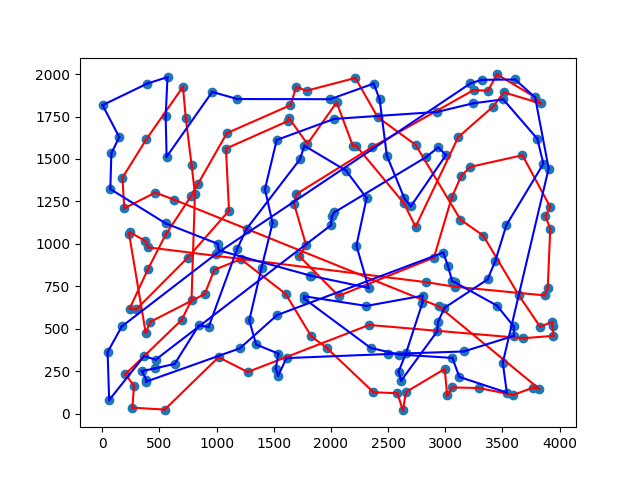
\includegraphics[width=\linewidth]{best_paths/kroB200/traverse_greedy_vertex/randomstart}
        \caption{kroB200, losowy start}
    \end{minipage}

    \vspace{0.5cm}

    % --- Drugi rząd ---
    \begin{minipage}[t]{0.45\textwidth}
        \centering
        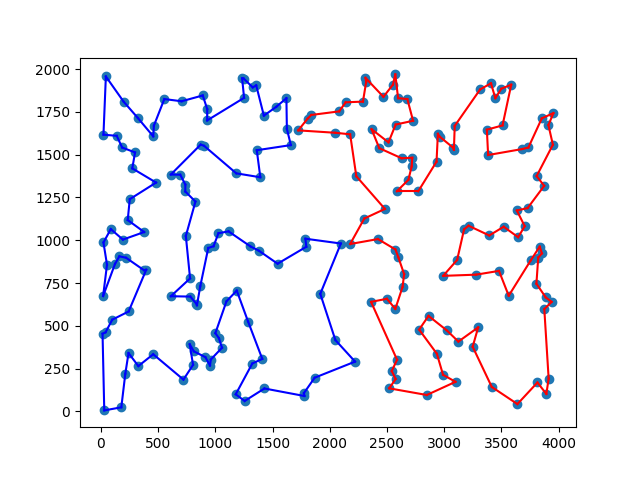
\includegraphics[width=\linewidth]{best_paths/kroA200/traverse_greedy_vertex/split_paths_regret_TSP}
        \caption{kroA200, własny algorytm startowy}
    \end{minipage}
    \hfill
    \begin{minipage}[t]{0.45\textwidth}
        \centering
        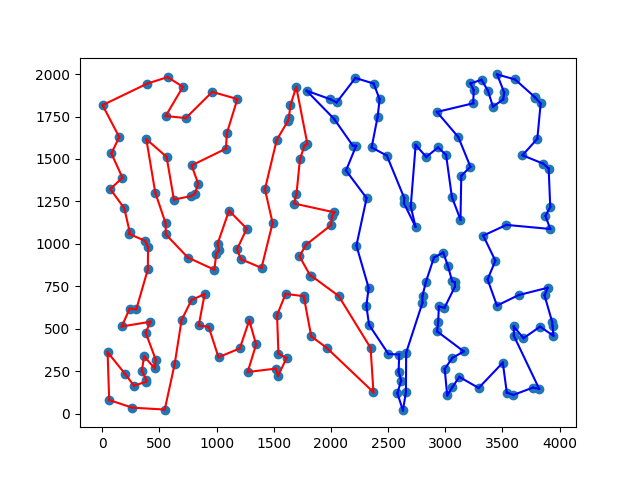
\includegraphics[width=\linewidth]{best_paths/kroB200/traverse_greedy_vertex/split_paths_regret_TSP}
        \caption{kroB200, własny algorytm startowy}
    \end{minipage}
    \label{fig:minipage-greedy-vertex}
\end{figure}

\subsubsection{Algorytm wymiany krawędzi (steepest)}
\begin{figure}[H]
    \centering
    % --- Pierwszy rząd ---
    \begin{minipage}[t]{0.45\textwidth}
        \centering
        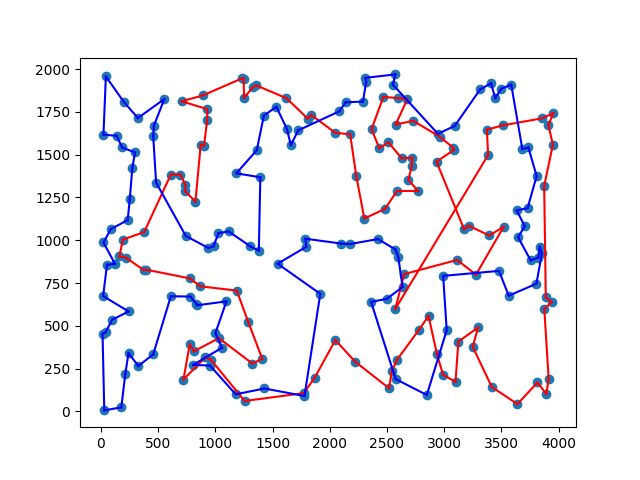
\includegraphics[width=\linewidth]{best_paths/kroA200/traverse_steepest_edge/randomstart}
        \caption{kroA200, losowy start}
    \end{minipage}
    \hfill
    \begin{minipage}[t]{0.45\textwidth}
        \centering
        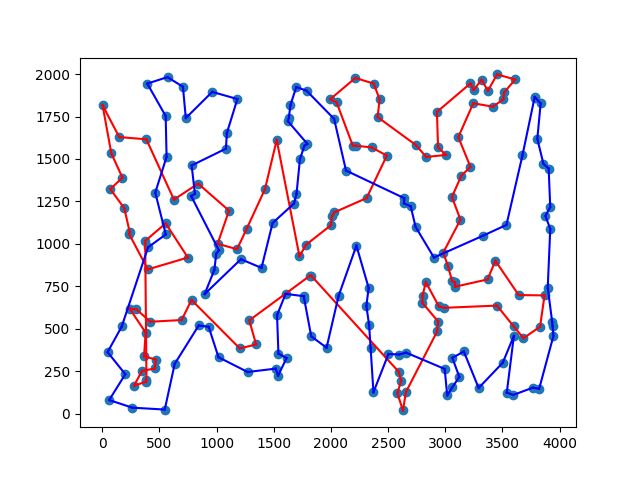
\includegraphics[width=\linewidth]{best_paths/kroB200/traverse_steepest_edge/randomstart}
        \caption{kroB200, losowy start}
    \end{minipage}

    \vspace{0.5cm}

    % --- Drugi rząd ---
    \begin{minipage}[t]{0.45\textwidth}
        \centering
        \includegraphics[width=\linewidth]{best_paths/kroA200/traverse_steepest_edge/split_paths_regret_TSP}
        \caption{kroA200, własny algorytm startowy}
    \end{minipage}
    \hfill
    \begin{minipage}[t]{0.45\textwidth}
        \centering
        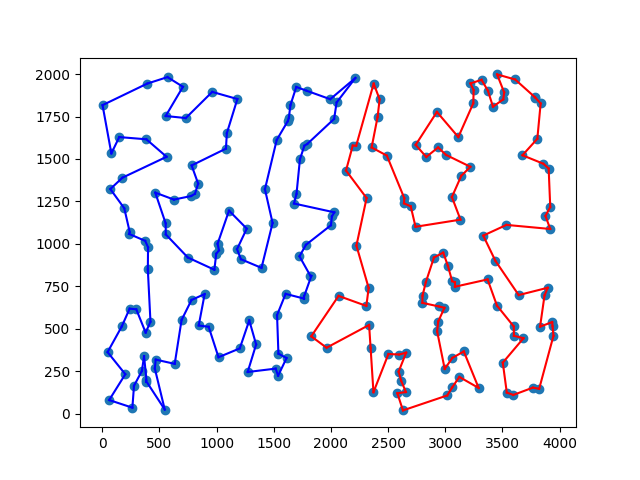
\includegraphics[width=\linewidth]{best_paths/kroB200/traverse_steepest_edge/split_paths_regret_TSP}
        \caption{kroB200, własny algorytm startowy}
    \end{minipage}
    \label{fig:minipage-steepest-edge}
\end{figure}


\subsubsection{Algorytm wymiany wierzchołków (steepest)}
\begin{figure}[H]
    \centering
    % --- Pierwszy rząd ---
    \begin{minipage}[t]{0.45\textwidth}
        \centering
        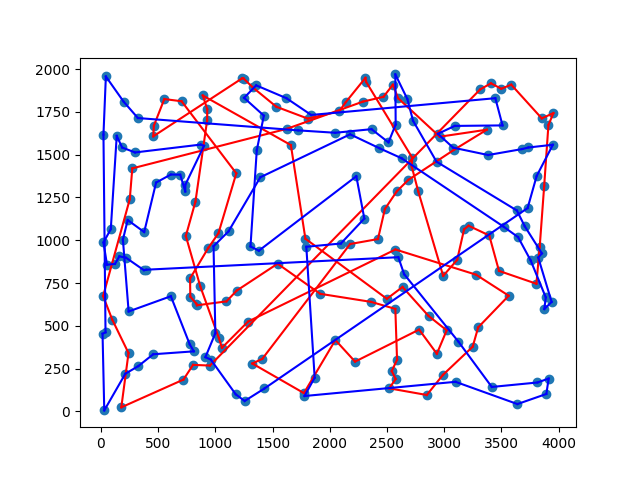
\includegraphics[width=\linewidth]{best_paths/kroA200/traverse_steepest_vertex/randomstart}
        \caption{kroA200, losowy start}
    \end{minipage}
    \hfill
    \begin{minipage}[t]{0.45\textwidth}
        \centering
        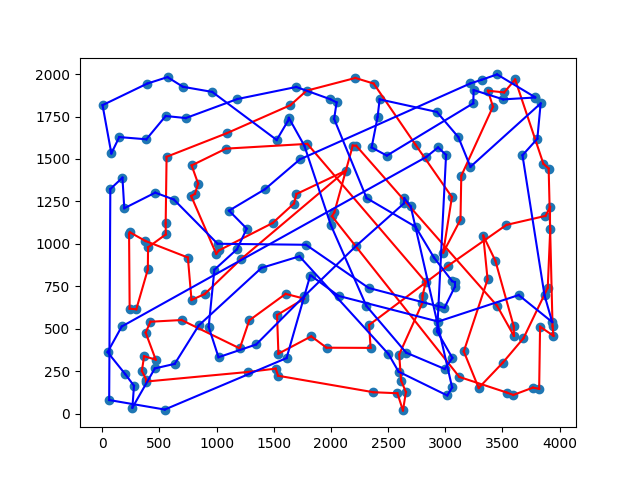
\includegraphics[width=\linewidth]{best_paths/kroB200/traverse_steepest_vertex/randomstart}
        \caption{kroB200, losowy start}
    \end{minipage}

    \vspace{0.5cm}

    % --- Drugi rząd ---
    \begin{minipage}[t]{0.45\textwidth}
        \centering
        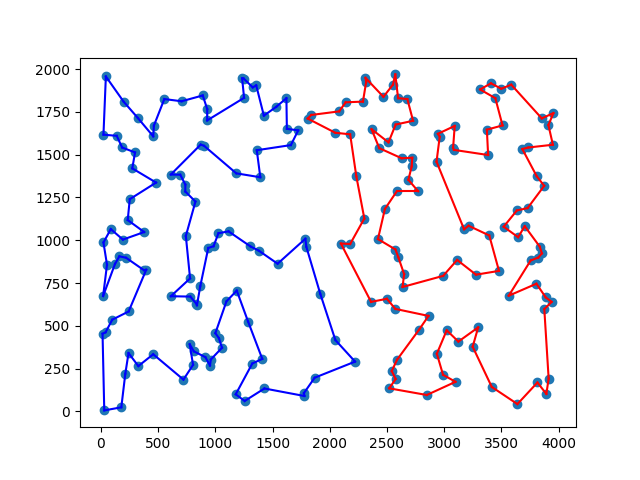
\includegraphics[width=\linewidth]{best_paths/kroA200/traverse_steepest_vertex/split_paths_regret_TSP}
        \caption{kroA200, własny algorytm startowy}
    \end{minipage}
    \hfill
    \begin{minipage}[t]{0.45\textwidth}
        \centering
        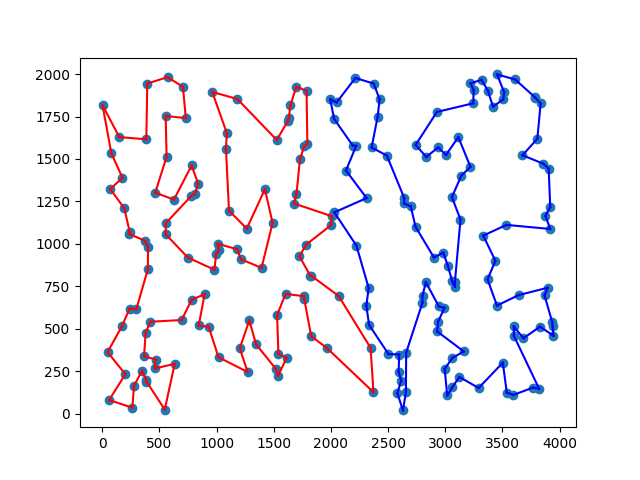
\includegraphics[width=\linewidth]{best_paths/kroB200/traverse_steepest_vertex/split_paths_regret_TSP}
        \caption{kroB200, własny algorytm startowy}
    \end{minipage}
    \label{fig:minipage-steepest-vertex}
\end{figure}


\subsubsection{Algorytm losowego błądzenia w  obu typach sąsiedztwa (random)}
\begin{figure}[H]
    \centering
    % --- Pierwszy rząd ---
    \begin{minipage}[t]{0.45\textwidth}
        \centering
        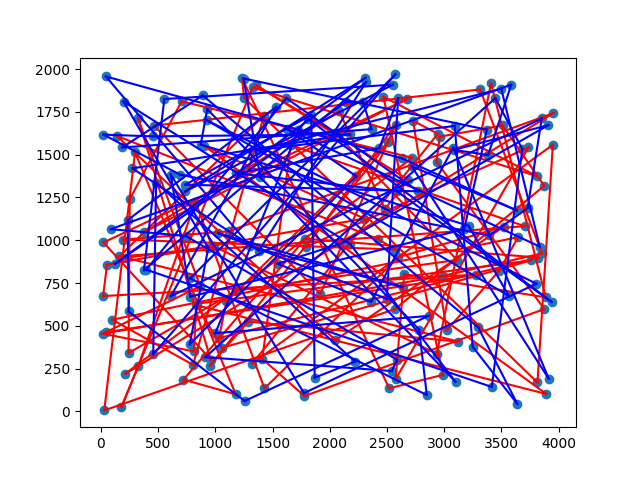
\includegraphics[width=\linewidth]{best_paths/kroA200/traverse_random/randomstart}
        \caption{kroA200, losowy start}
    \end{minipage}
    \hfill
    \begin{minipage}[t]{0.45\textwidth}
        \centering
        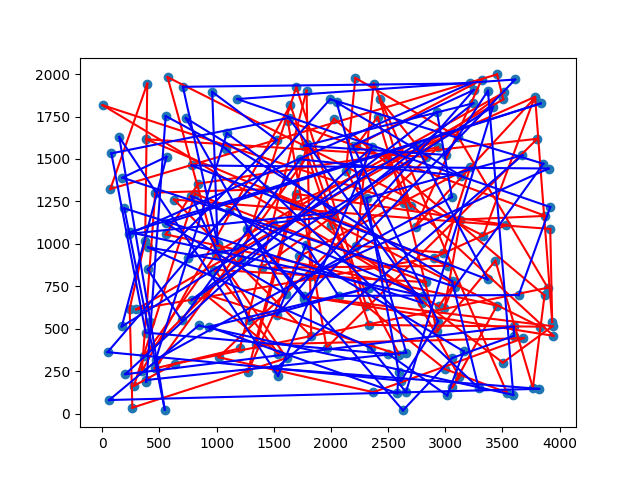
\includegraphics[width=\linewidth]{best_paths/kroB200/traverse_random/randomstart}
        \caption{kroB200, losowy start}
    \end{minipage}

    \vspace{0.5cm}

    % --- Drugi rząd ---
    \begin{minipage}[t]{0.45\textwidth}
        \centering
        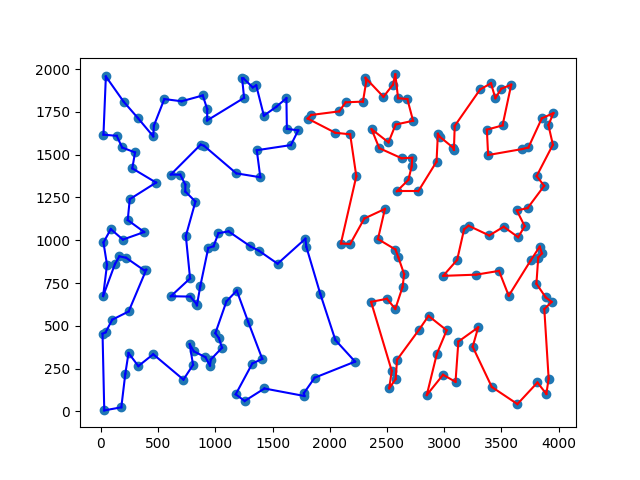
\includegraphics[width=\linewidth]{best_paths/kroA200/traverse_random/split_paths_regret_TSP}
        \caption{kroA200, własny algorytm startowy}
    \end{minipage}
    \hfill
    \begin{minipage}[t]{0.45\textwidth}
        \centering
        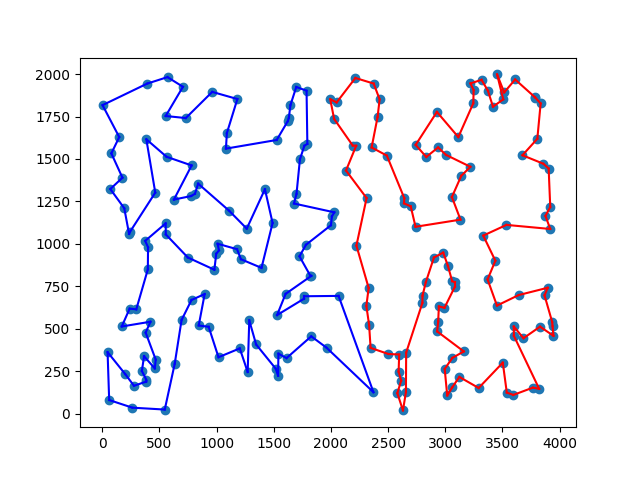
\includegraphics[width=\linewidth]{best_paths/kroB200/traverse_random/split_paths_regret_TSP}
        \caption{kroB200, własny algorytm startowy}
    \end{minipage}
    \label{fig:minipage-random}
\end{figure}

\section{Wnioski i analiza wyników}\label{sec:wnioski}

\begin{enumerate}
\item Algorytmy oparte na sąsiedztwie z zamianą krawędzi osiągnęły znacznie lepsze wyniki niż te oparte na zamianie wierzchołków.
\item Algorytmy steepest osiągały znacznie dłuższe czasy wykonywania, przynosząc jedynie niewielką poprawę co do jakości.
\item Pomimo świetnych wyników 2 tygodnie temu, okazuje się że nasz algorytm nadal da się poprawić, choć nie umiał zrobić tego algorytm losowego błądzenia.
Mimo to, wszystkie algorytmy osiągnęły jedynie niewielkie poprawy na startowym rozwiązaniu pozyskanym z naszego algorytmu.
\end{enumerate}


\section{Link do repozytorium}\label{sec:link-do-repo}
Kod źródłowy w repozytorium GitHub dostępny pod linkiem: \\
\href{https://github.com/KotZPolibudy/PUT_IMO/tree/main/Local_search}{Repozytorium Local Search}.

\end{document}
